\subsection{Ripianificazione a finire}

\subsubsection{Periodo di verifica e validazione}
Nel periodo di verifica e validazione la distribuzione oraria pianificata al //INSERIRE DATA// è la seguente:

\renewcommand{\arraystretch}{1.5}
\begin{table}[H]
\begin{center}
\begin{tabular}{|c|c|c|c|c|c|c|c|}
\hline
\rowcolor{title_row}
\textbf{\color{title_text}{Nome}} & \textbf{\color{title_text}{Resp.}} & \textbf{\color{title_text}{Ammi.}} & \textbf{\color{title_text}{Analist.}} & \textbf{\color{title_text}{Progett.}} & \textbf{\color{title_text}{Program.}} & \textbf{\color{title_text}{Verific.}} & \textbf{\color{title_text}{Totale}} \\ \hline
Andrea Trevisin  & & 6 & & & 7 & 9 & 22  \\ \hline
Giacomo Barzon   & & & & 7 & 6 & 6 & 19  \\ \hline
Giovanni Sorice  & & 8 & &  & 5 & 6 & 19  \\ \hline
Lorenzo Busin    & & & & & 8 & 10 & 18  \\ \hline
Marco Costantino & & 7 & & & 7 & 8 & 22  \\ \hline
Michele Roverato & & & & 7 & 7 & 8 & 22  \\ \hline
Nicolò Tartaggia & 10 & & & 6 & 3 & & 19  \\ \hline
\end{tabular}
\caption{Tabella 5.5.1: Distribuzione oraria del periodo "Verifica e validazione"\label{}}
\end{center}
\end{table}
\renewcommand{\arraystretch}{1}

Il seguente grafico dà una rappresentazione visiva della suddivisione oraria: \\
\begin{figure} [H]
	\centering
	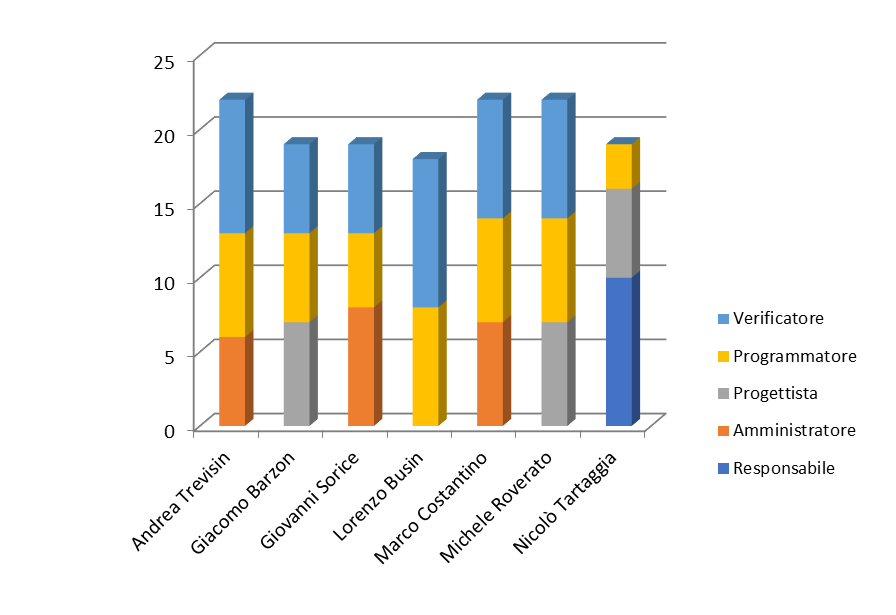
\includegraphics[scale=1]{Res/ExcelGrafici/Grafici/RipianificazioneOre.png}
	\caption{Figura 5.5.1: Grafico suddivisione oraria del periodo "Verifica e validazione"}\label{}
\end{figure}


\subsubsection{Prospetto economico}
Nel periodo di verifica e validazione il resoconto della distribuzione delle ore e dei relativi costi ripinaiificati è la seguente:

\renewcommand{\arraystretch}{1.5}
\begin{table}[H]
\begin{center}
\begin{tabular}{|c|c|c|}
\hline
\rowcolor{title_row}
\textbf{\color{title_text}{Ruolo}}  & \textbf{\color{title_text}{Ore}} & \textbf{\color{title_text}{Costo in \euro}} \\ \hline
Responsabile    & 10 & 300 \\ \hline
Amministratore  & 21 & 420 \\ \hline
Analista        & & \\ \hline
Progettista     & 20 & 440 \\ \hline
Programmatore   & 43 & 645 \\ \hline
Verificatore    & 47 & 705 \\ \hline
\textbf{Totale} & \textbf{141}    & \textbf{2.510}           \\ \hline
\end{tabular}
\caption{Tabella 5.5.2: Prospetto economico del periodo "Verifica e validazione"\label{}}
\end{center}
\end{table}
\renewcommand{\arraystretch}{1}

Il seguente grafico dà una rappresentazione visiva della distribuzione dei ruoli: \\
\begin{figure} [H]
	\centering
	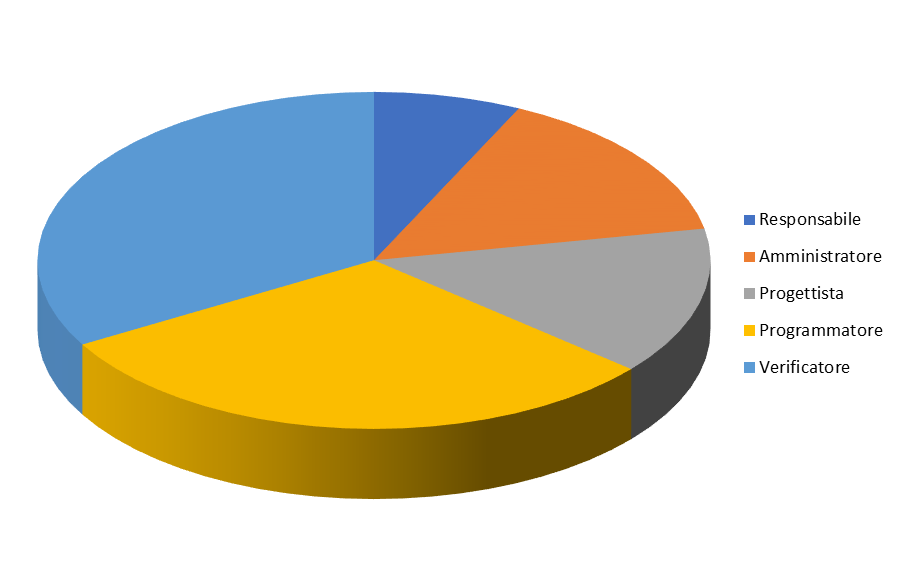
\includegraphics[scale=1]{Res/ExcelGrafici/Grafici/RipianificazioneRuoli.png}
	\caption{Figura 5.5.2: Grafico suddivisione dei ruoli del periodo "Verifica e validazione"}\label{}
\end{figure}

\pagebreak
